\include{preambel.tex}
\begin{document}
%===================Titlepage==============================
\thispagestyle{empty}
\newgeometry{left=2cm, right=2cm, top=2cm, bottom=2cm}
\begin{center}
\resizebox{0.4\textwidth}{!}{\itshape\textarabic{﷽}}\\[4ex]
{\Huge
العنوان
\\ 
}

%\begin{figure}[h!] %a decorative border. To get it, take it from tsunnah.
%\centering
%    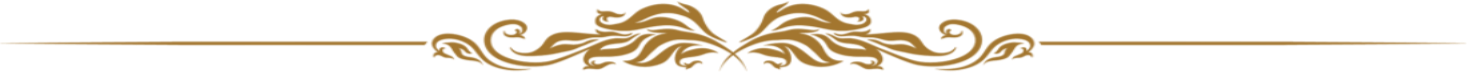
\includegraphics[width=0.9\textwidth]{fig/border_golden_5.png}
%\end{figure}

\vspace{11ex}

{\huge
    المعلم أو ما شابهه
}

\vspace{4ex}

%\begin{figure}[h!] %a logo
%    \centering
%    \includegraphics[width=0.4\textwidth]{fig/logo.jpg}
%\end{figure}

\vspace{8ex}

{\Large
الطالب: عبد الرحمن علي الشباك
}

%\vspace{80pt}
\vfill

{\Large
    ابتداء الدرس أو ما شابهه
}


\end{center}

%==================Table of Contents=======================
\restoregeometry
\newpage
{\hypersetup{ 
linkcolor=black
}
\thispagestyle{empty}
\tableofcontents
\newpage
\setcounter{page}{1}
}
    

%==================CONTENT=======================

\cleardoublepage
\setcounter{page}{1}
\include{01_Einfuehrung}

%==================Bibliography==================
%\nocite{*}
%\printbibliography

\printbibheading[
	heading=bibintoc
	]
\printbibliography[
	heading=subbibintoc,
	notkeyword=database, 
	nottype=book,
%	type=article
	heading=subbibliography,
	title={Wissenschaftliche Arbeiten}
	]
\printbibliography[
	heading=subbibintoc,
	keyword=database,
	nottype=article,
	heading=subbibliography,
	title={Datenbanken}
	]
\printbibliography[
	heading=subbibintoc,
	notkeyword=database,
	type=book,
	heading=subbibliography,
	title={Lehrb\"ucher}
	]
%\printbibliography[ %TODO in bib file (not citavi) \- in the isbn where too long, after everything else is done in sha Allah
%	heading=subbibintoc,
%	notkeyword=database,
%	notkeyword=dissertation,
%	nottype=article,
%	nottype=book,
%	heading=subbibliography,
%	title={Sonst.}
%	]

\include{08_Danksagung}


\newpage
\section{Eigenst\"andigkeitserkl\"arung}
Hiermit erkl\"are ich, dass ich die vorliegende Arbeit selbstst\"andig verfasst und keine anderen als die angegebenen Quellen und Hilfsmittel benutzt habe.

Alle sinngem\"a\ss{} und w\"ortlich \"ubernommenen Textstellen aus fremden Quellen wurden kenntlich gemacht.

Kassel, den 15. Februar 2021

\vspace{30pt}
Abdulrahman Shubbak
\end{document}

